% Gemini theme
% https://github.com/anishathalye/gemini

\documentclass[final]{beamer}

% ====================
% Packages
% ====================

\usepackage[T1]{fontenc}
\usepackage{lmodern}
\usepackage[size=custom,width=106.68,height=60.96,scale=0.85]{beamerposter}
\usetheme{custom}
\usecolortheme{tntech}
\usepackage{graphicx}
\usepackage{booktabs}
\usepackage{tikz}
\usepackage{pgfplots}
\usepackage{pgf}
\usepackage{multicol}
\usepackage{mathtools}

% ====================
% Lengths
% ====================

% If you have N columns, choose \sepwidth and \colwidth such that
% (N+1)*\sepwidth + N*\colwidth = \paperwidth
\newlength{\sepwidth}
\newlength{\colwidth}
\setlength{\sepwidth}{0.025\paperwidth}
\setlength{\colwidth}{0.3\paperwidth}

\newcommand{\separatorcolumn}{\begin{column}{\sepwidth}\end{column}}

\newcommand{\minus}{\scalebox{0.75}[1.0]{$-$}}
\newcommand{\smallequals}{\scalebox{0.75}[1.0]{$=$}}
\newcommand{\sectionHeading}[1]{\vskip2.0ex \textbf{#1} \vskip0.25ex}

% ====================
% Title
% ====================

\logotitle{
\includegraphics[height=5.0cm]{tntechgold.png}}
\title{SECON 2025 Hardware Competition Robot}
\author{Sean Borchers, Alex Cruz, Samuel Hunter, and Dakota Moye}
\institute[shortinst]{Tennessee Technological University}

% ====================
% Body
% ====================

\pgfplotsset{compat=1.16}
\begin{document}

\begin{frame}[t]
\begin{columns}[t]
\separatorcolumn

\begin{column}{\colwidth}

  \begin{block}{Introduction}

    \sectionHeading{Problem}
    
        The Institute of Electrical and Electronics Engineers (IEEE) hosts a yearly hardware competition at its Southeast Conference (SECON). Tennessee Technological University assembled a team to compete in the 2025 Hardware Competition with the objective of designing and constructing an autonomous robot. This robot would need to collect and sort randomly distributed material spread across a field over a 3-minute time frame. The material is sorted based on whether it is magnetic or not. The sorted material is stored in two plastic containers on the field, which are then sent to designated pads. The goal of the design process was to focus on reliably obtaining as many points as possible and having an extensive testing period to reduce runtime inconsistencies.
    
    \sectionHeading{Constraints}
    
1. The robot must fit within a 12x12x12 inch space at the starting position.

2. The robot must not exceed 12 kg.

3. The robot must contain a start button or mechanism.

4. The robot emergency stop button must be clearly visible and accessible.

5. The robot must not damage the field.

6. The power system of the robot must be 30 volts or less.


  \end{block}

  \begin{figure}
      \centering
      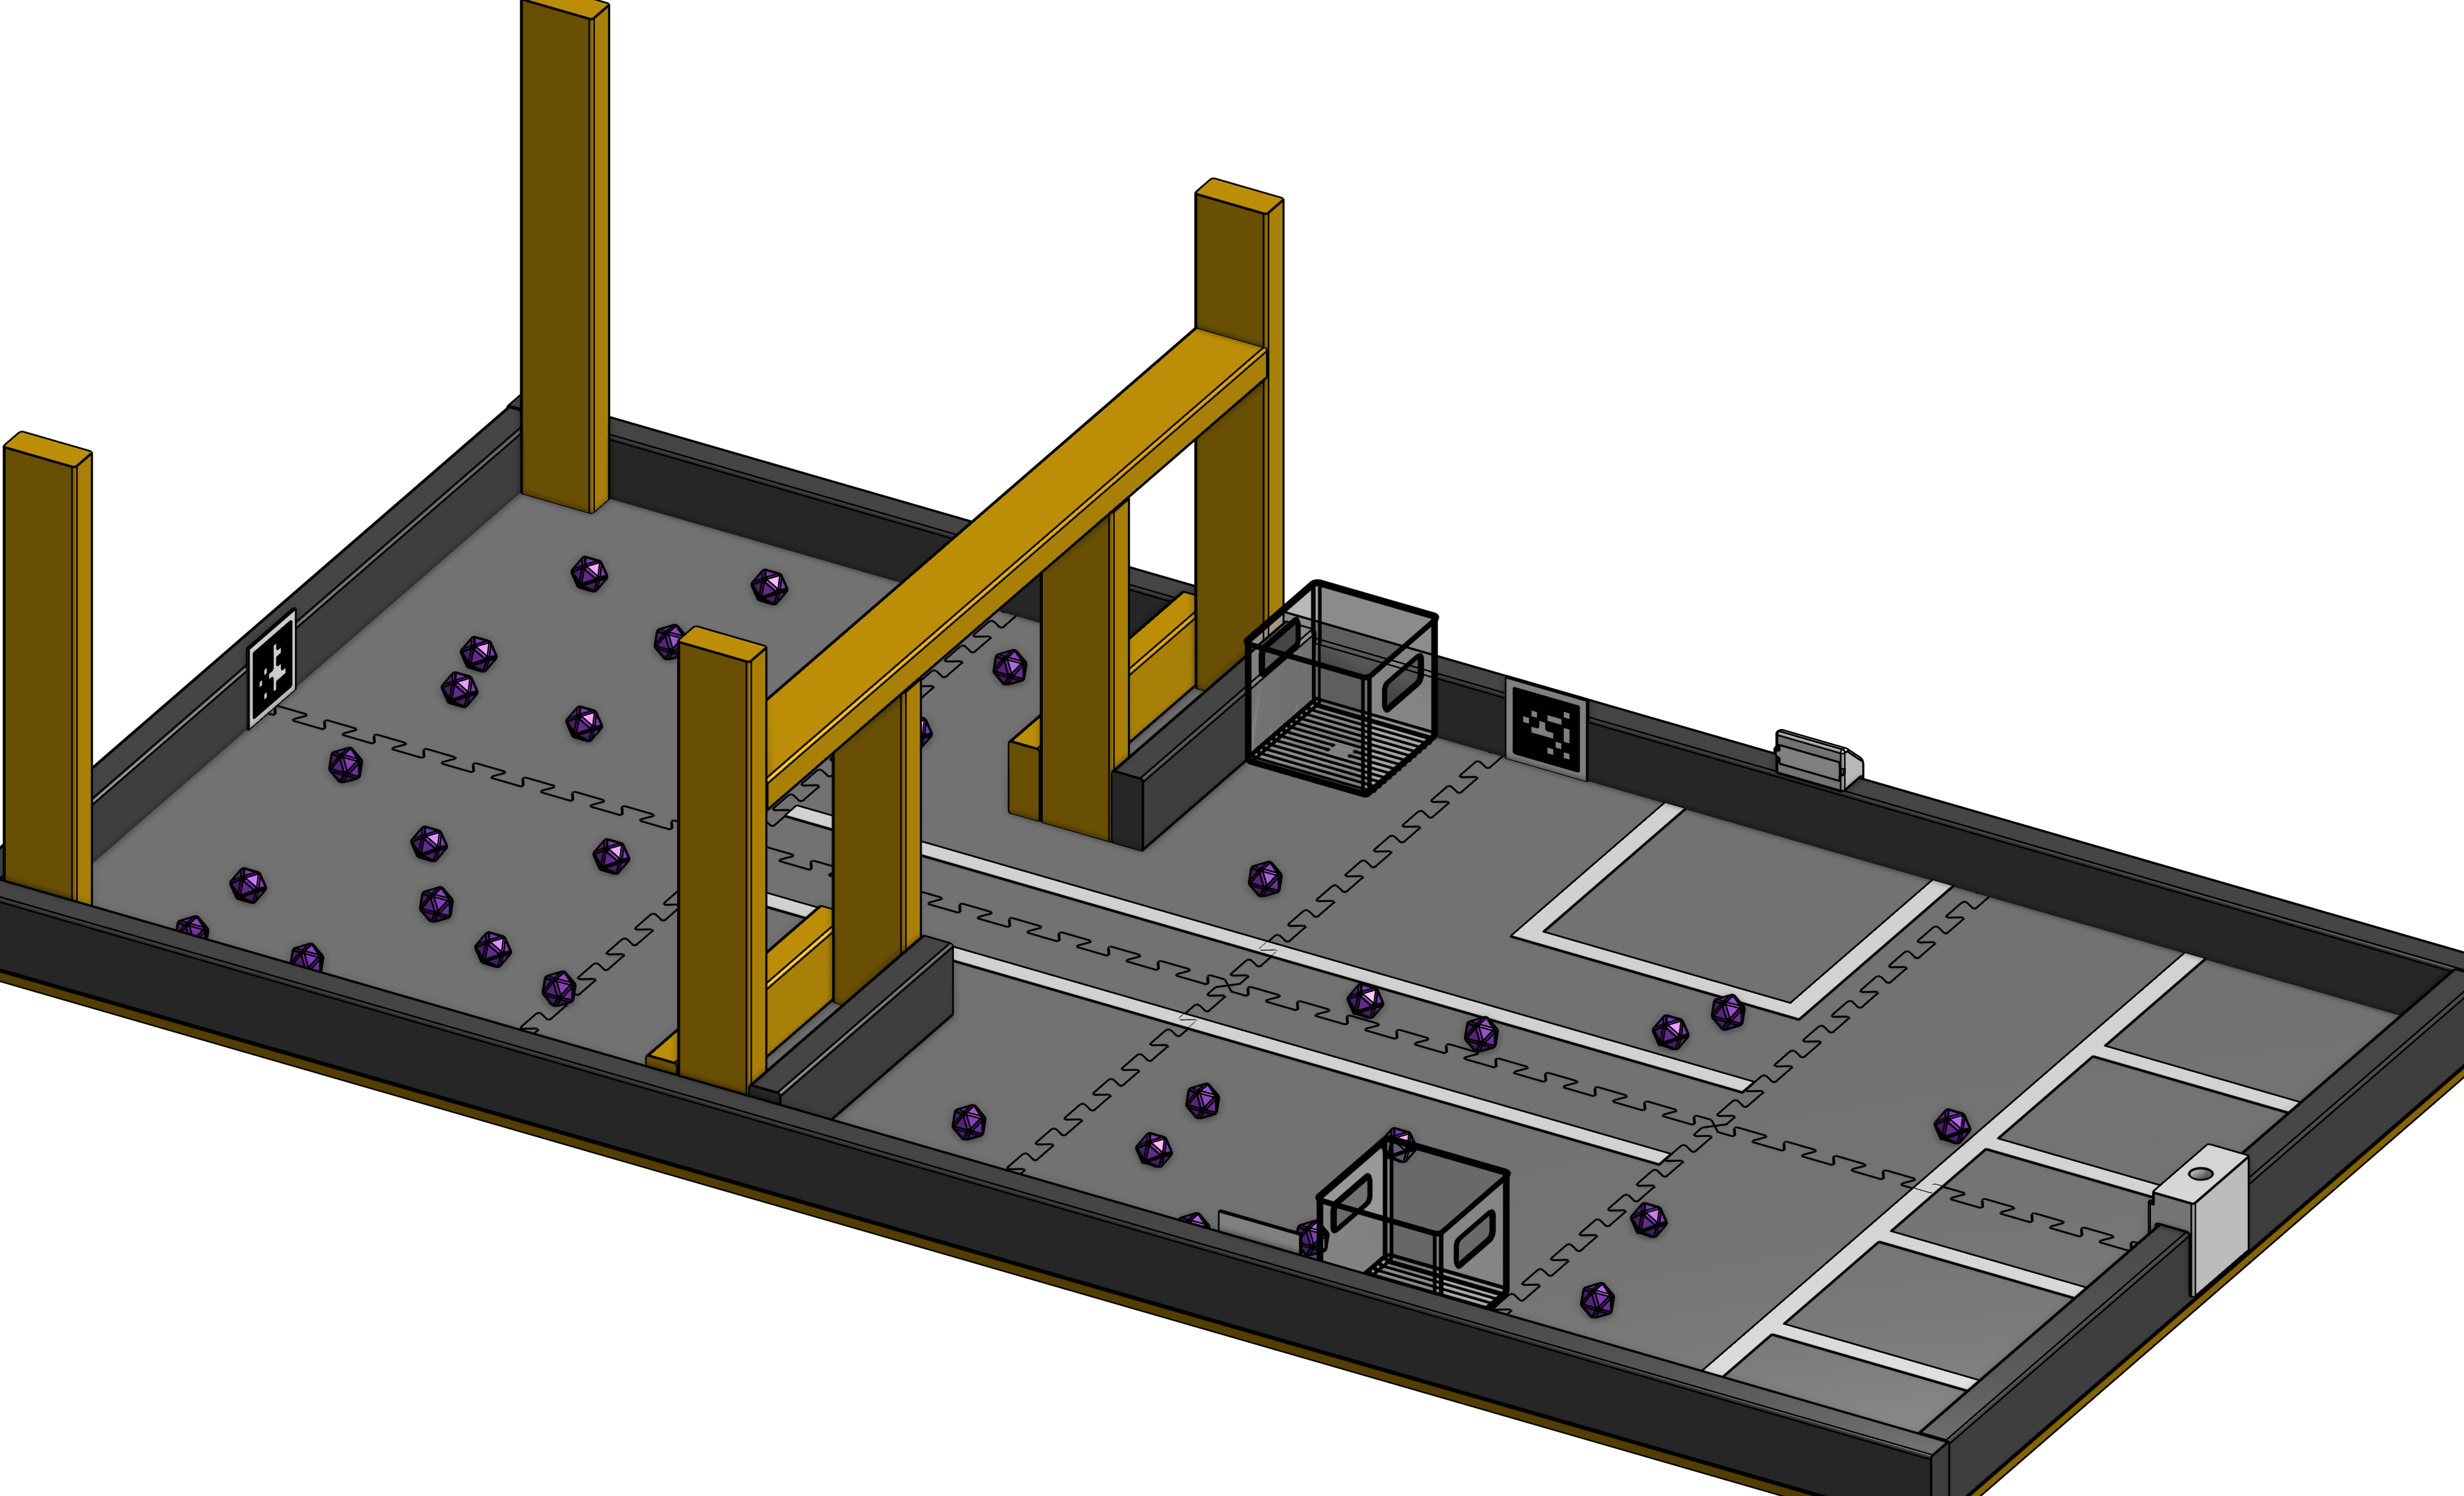
\includegraphics[width=20.0cm]{Mining Mayhem Field Opposite Corner.png}
      \caption{Game Field to compete on.}
    \end{figure}

  \begin{block}{Design}
    \begin{itemize}
    
      \item \textbf{Navigation}
        \begin{itemize}
          \item The robot navigates autonomously using orientation sensing.
        \end{itemize}
        
      \item \textbf{Motor Control}
        \begin{itemize}
          \item The motor control subsystem includes the design and operation of the motors for the robot wheels, arms, and other mechanisms that move based on sensor input and navigational commands. This subsystem would be considered lower-level robot control, as it explicitly includes details about certain motor speeds and directions for when specific conditions are met during play.
        \end{itemize}
      
      \item \textbf{Camera}
        \begin{itemize}
          \item The camera detects objects and symbols.
        \end{itemize}
      
      \item \textbf{Sensors}
        \begin{itemize}
          \item The sensors subsystem is able to detect orientation, magnetic fields, and light levels. This information is then provided to the controllers for processing. The sensors subsystem is always active for when the controller needs information. Orientation sensor provides information about the robot's current position which way it is facing. The magnetic sensors detect if there is a magnetic field in specific materials. The light sensors detect a difference in light levels.
        \end{itemize}
    
    \end{itemize}
  
  \end{block}

    % \begin{figure}
    %   \centering
    %   
\includegraphics[width=20.0cm]{Neuron.png}
    %   \caption{Neuron Diagram}
    % \end{figure}


    
    % \begin{figure}
    %   \centering
    %   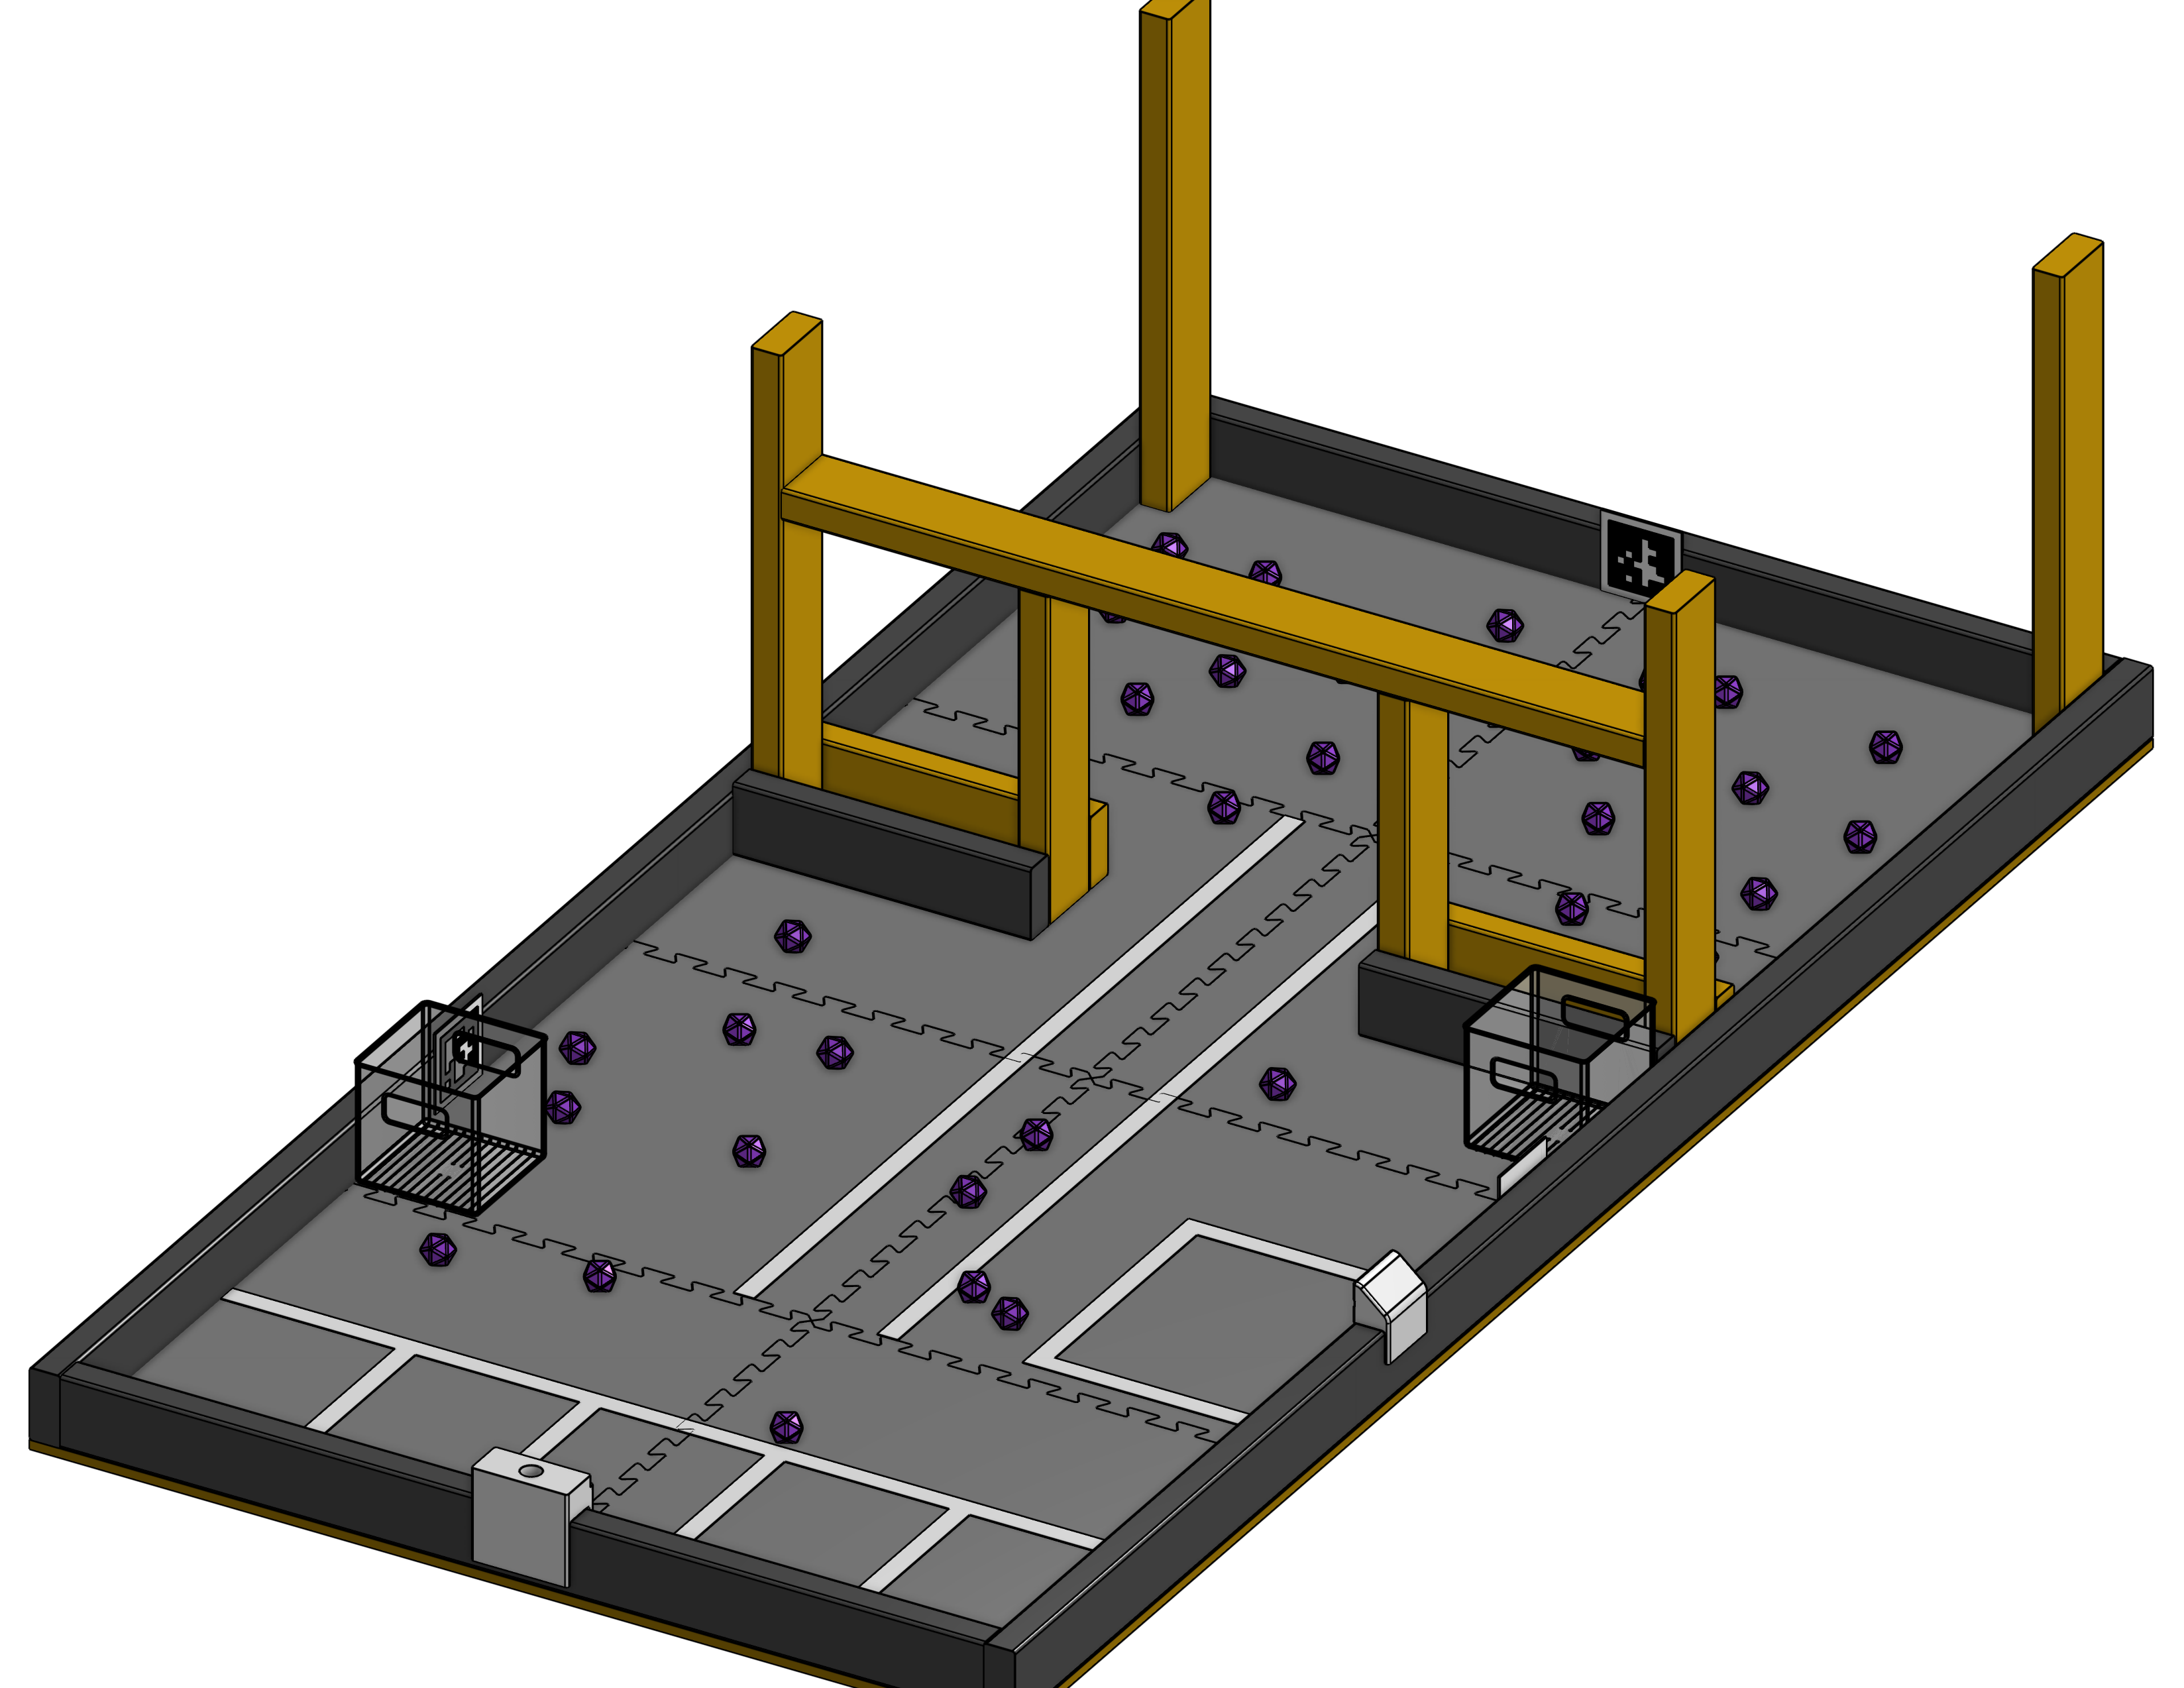
\includegraphics[width=20.0cm]{Mining Mayhem Field.png}
    %   \caption{Game Field to compete on.}
    % \end{figure}

\end{column}

\separatorcolumn

\begin{column}{\colwidth}

    \begin{figure}
      \centering
      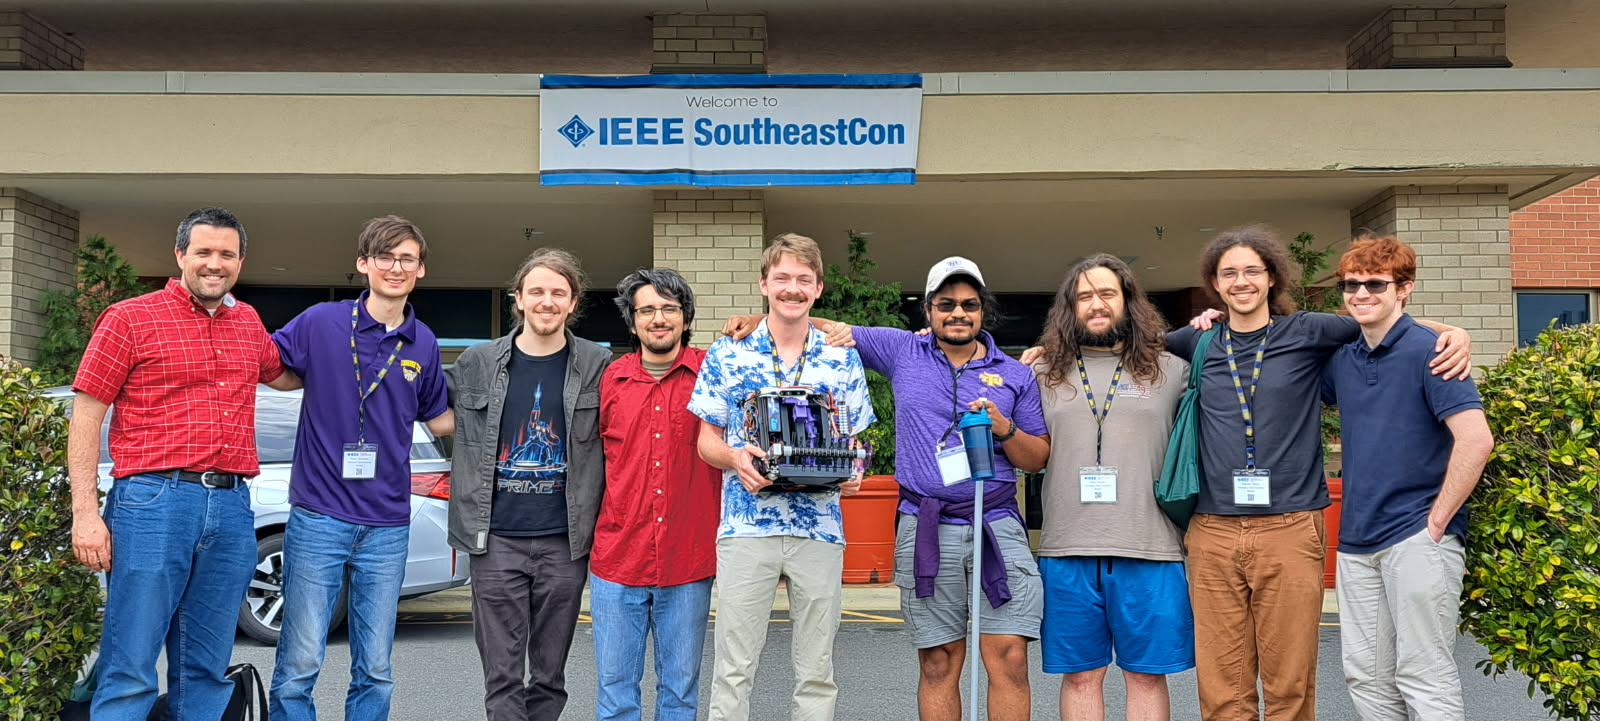
\includegraphics[width=30.0cm]{Team Picture SECON 2025.jpg}
      \caption{Micah Rentschler, Sean Borchers, Caleb Sullivan, Alex Cruz, Cooper Nelson, Phoenix Sims, Sam Hunter, Dakota Moye, Nick Moulton}
    \end{figure}

    \begin{figure}
      \centering
      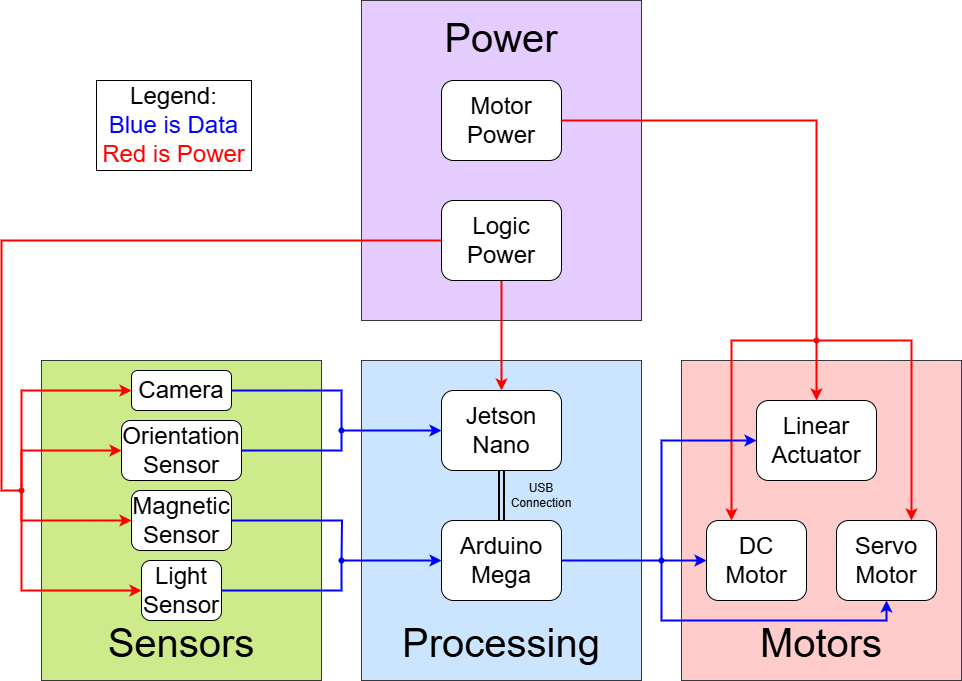
\includegraphics[width=20.0cm]{High_Block_Diagram.png}
      \caption{High Level Block Diagram.}
    \end{figure}

\end{column}

\separatorcolumn

\begin{column}{\colwidth}

    \begin{block}{Experimentation}

    Robo does everything to a degree.

  \end{block}

  \begin{figure}
      \centering
      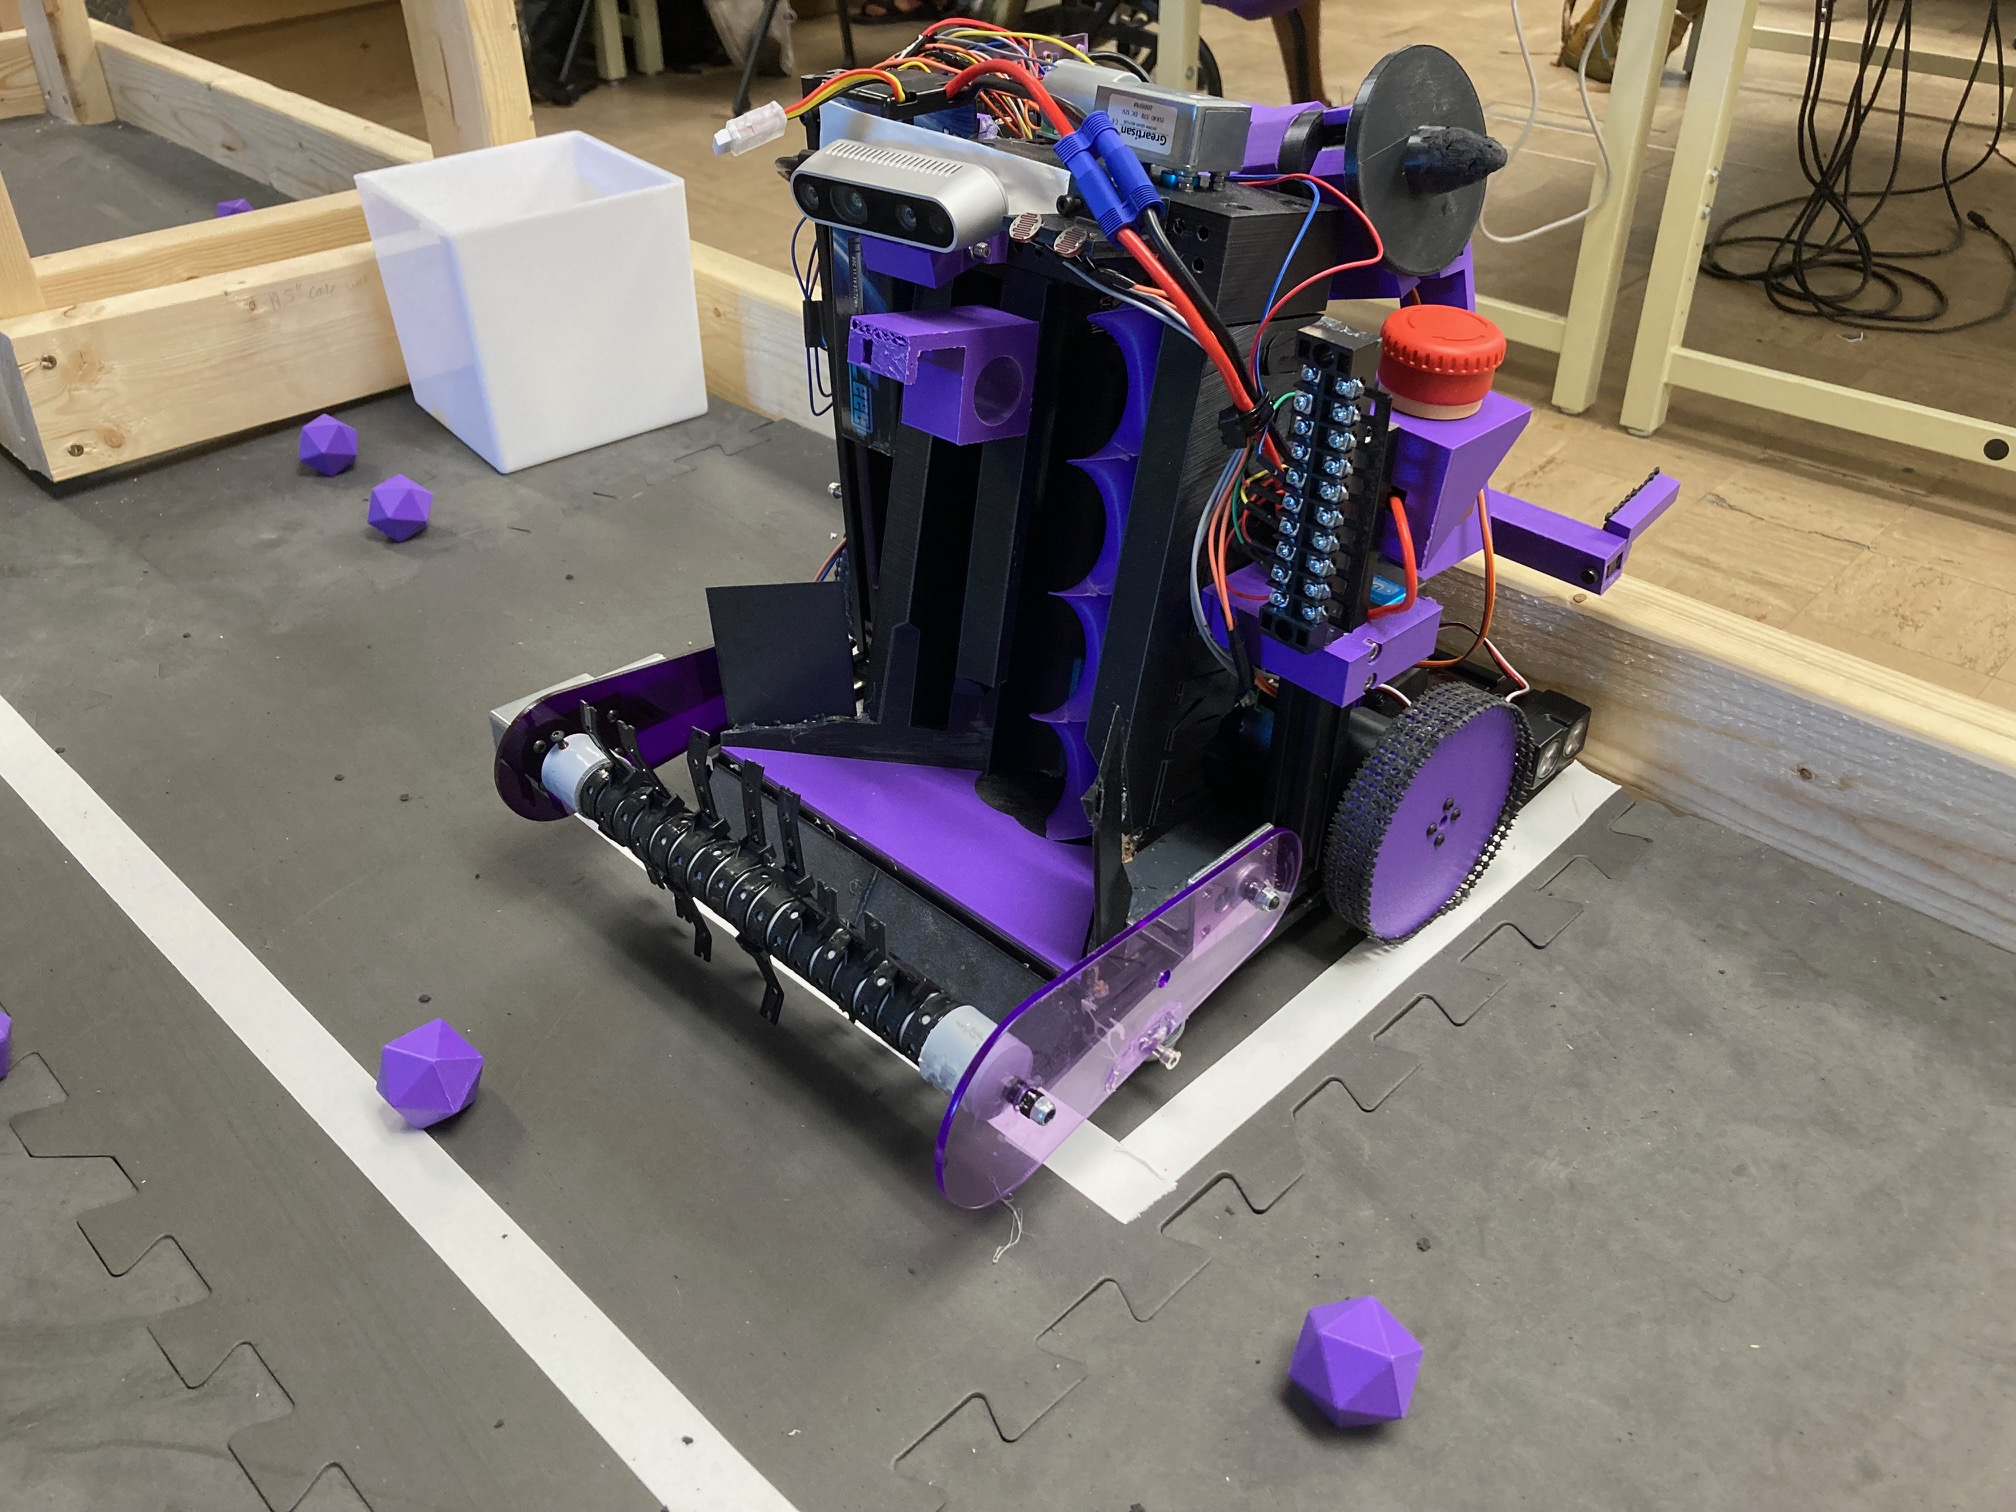
\includegraphics[width=20.0cm]{Robot_Practice_Field.jpg}
      \caption{Final Robot Product}
    \end{figure}

  \begin{block}{Conclusion}
    Put BOM and final thoughts here.

    % start example table

    % \begin{columns}[t]
    %   \begin{column}{0.4\colwidth}

    %     \begin{table}[ht]
    %       % increase table row spacing, adjust to taste
    %       \caption{Gen 1 ANN Model Assumptions}
    %       \label{Table:Gen1ANNAssumptions}
    %       \centering
    %       % Some packages, such as MDW tools, offer better commands for making tables
    %       % than the plain LaTeX2e tabular which is used here.
    %       \resizebox{\columnwidth}{!}{%
    %       \begin{tabular}{ c l }
    %         \toprule
    %         \textbf{Number} & \textbf{Assumption}\\
    %         \midrule
    %         1 & Firing Frequency Encoding\\

    %         2 & Steady State\\

    %         3 & Unity Static Firing Rate\\

    %         4 & Learned Inhibition\\

    %         5 & Unconditional Weighting\\
    %        \bottomrule
    %       \end{tabular}}
    %     \end{table}
    %   \end{column}

    %   \begin{column}{0.4\colwidth}
    %     \begin{table}[ht]
    %       % increase table row spacing, adjust to taste
    %       \caption{Gen 2 ANN Model Assumptions}
    %       \label{Table:Gen2ANNAssumptions}
    %       \centering
    %       % Some packages, such as MDW tools, offer better commands for making tables
    %       % than the plain LaTeX2e tabular which is used here.
    %       \resizebox{\columnwidth}{!}{%
    %       \begin{tabular}{ c l }
    %         \toprule
    %         \textbf{Number} & \textbf{Assumption}\\
    %         \midrule
    %         1 & Firing Frequency Encoding\\

    %         2 & Steady State\\

    %         3 & Learned Inhibition\\

    %         4 & Unconditional Weighting\\
    %         & \\
    %         \bottomrule
    %       \end{tabular}}
    %     \end{table}
    %   \end{column}

    % \end{columns}

    % end example table
    
  \end{block}

\end{column}

\separatorcolumn
\end{columns}
\end{frame}

\end{document}
